\documentclass{beamer}

\usepackage[utf8x]{inputenc}
\usepackage[british,russian]{babel}
\usepackage{graphicx,hyperref,ru,url}

% The title of the presentation:
%  - first a short version which is visible at the bottom of each slide;
%  - second the full title shown on the title slide;
\title[ППП. Задание 2]{
  Пакеты прикладных программ. Весна 2017}

% Optional: a subtitle to be dispalyed on the title slide
\subtitle{Задание №2}

% The author(s) of the presentation:
%  - again first a short version to be displayed at the bottom;
%  - next the full list of authors, which may include contact information;
\author[Кафедра ИО]{
    Комиссаров Александр \\
    Максимов Пётр \\
    Облыгина Олеся
  }

% The institute:
%  - to start the name of the university as displayed on the top of each slide
%    this can be adjusted such that you can also create a Dutch version
%  - next the institute information as displayed on the title slide
\institute[МГУ им. М.В. Ломоносова]{
  Московский Государственный Университет им. М.В. Ломоносова \\
  Факультет Вычислительной Математики и Кибернетики\\
  Кафедра Исследований Операций}

% Add a date and possibly the name of the event to the slides
%  - again first a short version to be shown at the bottom of each slide
%  - second the full date and event name for the title slide
\date[Апрель 2017]{
   \\
  Апрель 2017}

\begin{document}

\begin{frame}[plain]
    \titlepage  
\end{frame}
  
\begin{frame}
  \frametitle{Содержание}

  \tableofcontents
\end{frame}

% Section titles are shown in at the top of the slides with the current section 
% highlighted. Note that the number of sections determines the size of the top 
% bar, and hence the university name and logo. If you do not add any sections 
% they will not be visible.
\section{Постановка задачи}

\begin{frame}
  \frametitle{Постановка задачи}
  
  Мы выступаем в качестве аналитика Дейнерис Бурерожденной из дома
  Таргариенов, Неопалимой, Кхалиси, Матери Драконов и пр. пр., и помогаем её советнику Тириону Ланистеру выбрать для армии Безупречных поставщика.
   
\end{frame}

\begin{frame}
  \frametitle{Постановка задачи}

    Необходимо по заданным данным (количество произведенных мечей и брака за каждый прошедший месяц) понять и обосновать, какая компания по производству стали лучше:
    
    \
    
    \begin{minipage}{0.3\textwidth}
        \begin{itemize}
            \item Harpy\&Co
        \end{itemize}
        
        \hspace{20pt}
        
\includegraphics[scale = 0.1]{game_of_thrones_son_of_the_harpy.png}
    \end{minipage}
    \begin{minipage}{0.3\textwidth}
        \begin{itemize}
            \item Westeros Inc.
        \end{itemize}
        
        \hspace{20pt}
        
\includegraphics[scale = 0.07]{iron_throne.png}
    \end{minipage}
       
\end{frame}


\section{Извлечение данных}

\begin{frame}
  \frametitle{Извлечение данных}
    Для начала нам необходимо разобраться, какие данные что означают, и как их обрабатывать: \
    
    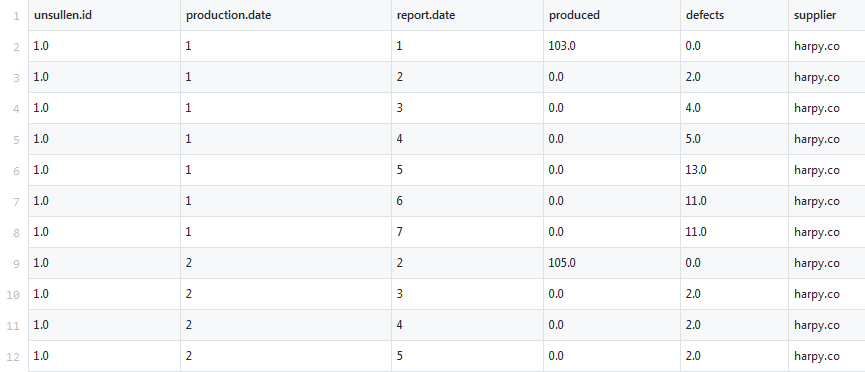
\includegraphics[scale = 0.5]{data.PNG}
\end{frame}

\begin{frame}
    \frametitle{Извлечение данных}
    Вполне очевидно, что первый столбец это номер кузнеца, а последний - компания поставщик. 
    
    Будем считать, что production.date это номер произведенной партии от данного кузнеца; report.date - месяц отчета по этой партии; produced - параметр отчета, т.е. количество произведенных мечей; defects - также параметр отчета, только уже количество сломанных мечей. 
    
\end{frame}

\begin{frame}
    \frametitle{Извлечение данных}
    
    Для обработки данных перенесём эти значения в объект Data.Frame и добавим две дополнительные характеристики, которые понадобятся нам в дальнейшем:
    \begin{block}{unbroken}
        Количество целых мечей для каждой партии
    \end{block}
    
    \begin{block}{broke\_per}
        Процент сломавшихся за последний месяц мечей к количеству оставшихся целых
    \end{block}
    
\end{frame}

\section{Регрессионный анализ}

\begin{frame}
    \frametitle{Анализ данных}
    Первоначально, для достоверного анализа мы должны убрать из рассмотрения эффекты, которые могут исказить представления о качестве поставляемой стали. Это могут быть личные качества каждого кузнеца, качества партий стали и какие-то временные происшествия (например, большое количество битв). Но по условию наши кузнецы все одинаковы и безупречны. Значит рассматривать мы будем только второй и третий эффекты.
  
\end{frame}


\begin{frame}
    \frametitle{Анализ. Улучшение статистики}
    Для визуализации временных происшествий и оценки этого параметра на данные мы произвели следующие действия:

    \begin{enumerate}
        \item Нашли средние значения сломавшихся мечей по каждому кузнецу (использовали тот самый broke\_per)
        \item Нашли среднее геометрическое значения процента сломавшихся мечей по времени использования меча
        \item Для каждой партии нашли отклонение от получившегося среднего
        \item Построили таблицу зависимостей сломавшихся мечей от месяца отчета и месяца производства (см. ниже)
    \end{enumerate}
\end{frame}

\begin{frame}
    \frametitle{Анализ. Построенная таблица}
    
    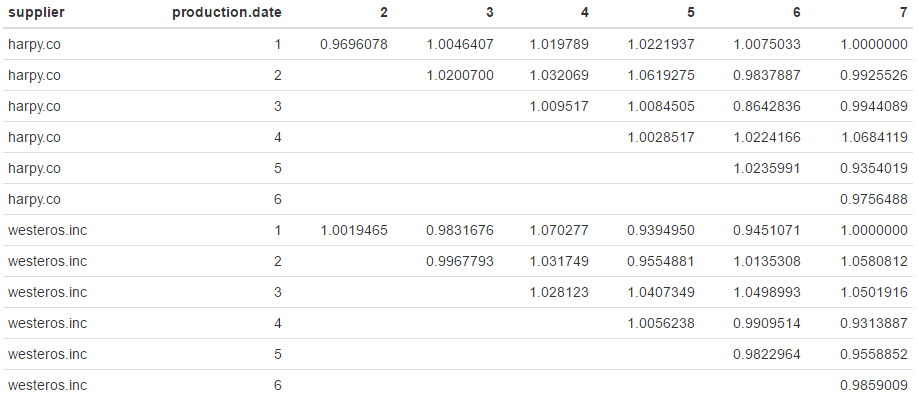
\includegraphics[scale = 0.46]{table.PNG}
    
\end{frame}

\begin{frame}
    \frametitle{Анализ. Выводы из таблицы}
    Невооруженным взглядом видно, что все значения близки к единице. Значит никаких ярких дефектов или происшествий не происходило за это время. Отлично, мы можем перейти к анализу данных без внешних возмутителей.
    
\end{frame}

\begin{frame}
    \frametitle{Прямой анализ}
    Для этого построим зависимость процента сломанных мечей от времени их использования по каждому производителю
    
    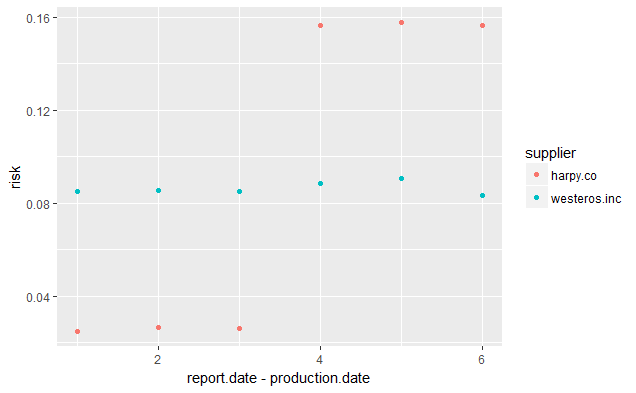
\includegraphics[scale = 0.5]{risk.png}
    
\end{frame}

\begin{frame}
    \frametitle{Анализ. Вывод}
    
    Получаем, что в Westeros Inc. вероятность поломки меча приблизительно постоянная по времени, а в Harpy\&Co первые три месяца низкая, а в следующие существенно возрастает и остается постоянной. Теперь мы можем перейти к прогнозу на следующие 11 месяцев.
\end{frame}

\section{Построение предсказания}

\begin{frame}
    \frametitle{Построение предсказания}
    Используя полученную нами модель построим предположение и визуализируем его:
    
    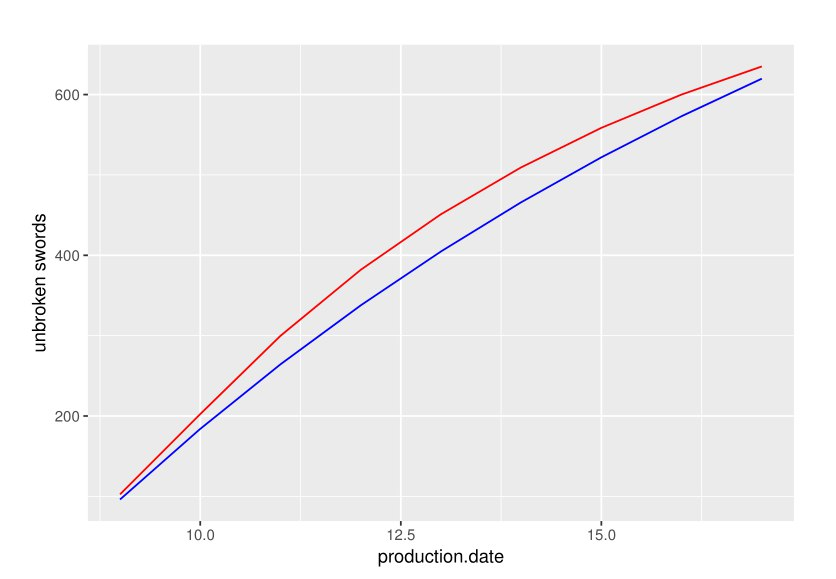
\includegraphics[scale = 0.4]{swords.png}
    
\end{frame}

\begin{frame}
    \frametitle{Предсказание. Вывод из графика}
    
    Красным обозначено Harpy\&Co, синим - Westeros Inc. 
    
    \
    
    По графику видно, что Harpy\&Co доминирует над Westeros Inc. по всему горизонту планирования, т.е. количество рабочих мечей у них всегда будет больше. Поэтому уже сейчас можно предположить, что эта компания лучше справится со своими обязанностями. Но для подтверждения результата введем еще одну числовую характеристику.
\end{frame}

\begin{frame}
    \frametitle{Предсказание. Численная характеристика}
    
    Новая характеристика представляет собой время работы всех мечей в течении горизонта планирования. Для каждой компании она равна:
    
    \begin{itemize}
        \item Harpy\&Co - 4.949132
        \item Westeros Inc. - 4.660751
    \end{itemize}
\end{frame}

\section{Заключение}

\begin{frame}
    \frametitle{Заключение}
    
    Получаем, что мечи из стали Harpy\&Co долговечнее в среднем на 0.3 месяца. Следовательно необходимо посоветовать именно эту компанию Тириону.
    
    \
    
    
\includegraphics[scale = 0.4]{Targaryen.png}
\end{frame}

\end{document}
